% !TeX spellcheck = de_DE

\chapter{GIS Verschneidung}


\section{Themen}

\subsection{Mögliche Fragestellungen}
\begin{itemize}
	\item Wie können Vektor und Rasterdaten miteinander verschnitten werden?
	\item Wie können aus der Verschneidung von Datensätzen neue Informationen gewonnen werden?
	\item Wie können Informationen von überlappenden Datensätzen in Mars genutzt werden?
	\item Wie kann ein Layer in MARS LIVE Daten mehrerer Layer aggregieren.
\end{itemize}


\subsection{Ausgeschlossene Themen}
\begin{itemize}
	\item Einfache Reduktion von 2 Vektorflächen auf die gemeinsame Fläche (Union) ist ein gelöstes Problem, dass von gängigen GIS Programmen unterstützt wird.
	\item Verbesserung von Verschneidungsalgorithmen, die seit Jahren nicht verbessert wurden ist wenig erfolgversprechend.
\end{itemize}



\section{Motivation}
Das MARS LIFE Simulationssystem benötigt für die Initialisierung verschiedene Typen von spatialen Daten. Die Aufbereitung der Daten obliegt dem Modellierer, der die Datensätze mit Hilfe spezieller GIS Software erstellen muss. Um die Arbeit mit MARS zu erleichtern, ist die automatisierte Informationsgewinnung aus kombinierten Datensätzen von zentraler Bedeutung.\\
Als Voraussetzung für die sog. Verschneidung müssen die Datensätze den selben geographischen Bereich abdecken. Darüber hinaus muss mit unterschiedlichen räumlichen Auflösungen und der Kombination von Vektoren und Rasterdaten umgegangen werden.


\subsection{Vorbereitung}
Für die Durchführung einer Verschneidung müssen folgende Verarbeitungsschritte im Vorfeld durchgeführt werden.

\subsubsection{Angleichung des Coordinate Reference System (CRS)}
Spatiale Daten bilden die Erde auf einer ebenen Fläche ab. Hierzu gibt es verschiedene Methoden, die abhängig von dem geographischem Gebiet unterschiedliche Ergebnisse liefern. Für die Verarbeitung müssen Daten auf eine gemeinsame Projektion gebracht werden. Für eine Gesamtansicht der Erde hat sich WGS84 als Standard etabliert.

\subsubsection{Reduktion von Datensätzen auf die ermittelte Überschneidungsfläche.}
Um Informationen aus verschiedenen Datensätzen zu gewinnen müssen die geographischen Bereiche identisch sein. Es muss also die gemeinsame Fläche berechnet und die übrigen Flächen ignoriert werden.
\begin{figure}[H]
	\centering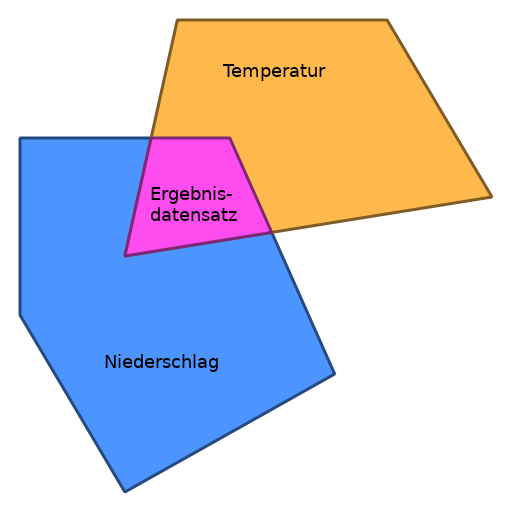
\includegraphics[width=0.5\textwidth]{res/Reduktionsbeispiel}
	\caption{Reduktionsbeispiel}
	\label{fig:Reduktionsbeispiel}
\end{figure}

\subsubsection{Räumliche Auflösung}
Datensätze können in unterschiedlichen räumlichen Auflösungen vorliegen. Für die Informationsgewinnung ist es notwendig, in Abhängigkeit zu der Art der Daten eine Interpolation durchzuführen. Hierbei dürfen möglichst keine Informationen verloren gehen. Sinnvoll wäre ein paar gängige interpolationsformeln zu unterstützen.


\subsection{Informationsgewinnung aus Verschneidung (Remote Sensing)}
Die Informationsgewinnung verschiedener spatialer Daten kann auf verschiedene Weise geschehen. Eine Möglichkeit ist, die des spatialen Indikators, wie sie von \cite{Baldowski2014} in Kapitel 5.4 seiner Masterarbeit beschrieben wurde (siehe Abb. \ref{fig:SGI}). Dieser Ansatz klassifiziert und addiert Werte in Rasterzellen. Das Ergebnis ist ein einfacher Zahlenwert.\\
Darüber hinausgehend wäre es denkbar Daten auf Basis von Formeln dynamisch zu verschneiden. So könnten aus Niederschlags- und Temperaturdaten die Fruchtbarkeit des Gebiets berechnet werden. Es wäre auch möglich aus Landnutzungskarten und einer Höhenkarte den optimalen Weg für Fortbewegung im Gelände zu berechnen.
\begin{figure}[H]
	\centering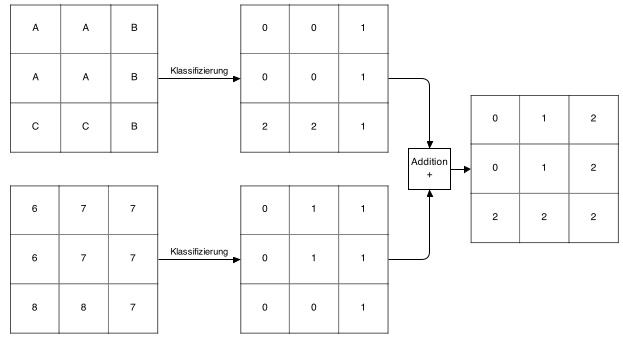
\includegraphics[width=.75\textwidth]{res/Verschneidung}
	\caption{Spatialer indikator nach \cite{Baldowski2014}}
	\label{fig:SGI}
\end{figure}


\section{Paper}
\begin{itemize}
	\item \textbf{A spatial data partitioning and merging method for parallel vector spatial analysis}: \cite{Qiu2015}
	\item \textbf{Räumliche Analyse mit spatialen Indikatoren}: \cite{Baldowski2014}
	\item \textbf{MapSnap system to perform vector-to-raster fusion}: \cite{Kovalerchuk2011}
	\item \textbf{Multi-source remote sensing data fusion: status and trends}: \cite{Zhang2010}
	\item \textbf{Mathematical support for combining geospatial data}: \cite{Kovalerchuk2001}
\end{itemize}
